\documentclass[letterpaper,11pt]{article}

% -------------------------
% PAQUETES
% -------------------------
\usepackage[spanish]{babel}
\usepackage[utf8]{inputenc}
\usepackage[T1]{fontenc}
\usepackage{graphicx}
\usepackage{geometry}
\usepackage{array}
\usepackage{setspace}
\usepackage{titlesec}
\usepackage{enumitem}
\geometry{margin=2.5cm}
\usepackage{amsmath}

\usepackage{float}
\usepackage{xcolor}
\usepackage{realboxes}
\definecolor{lightgrey}{rgb}{0.95,0.95,0.95} % El color del fondo

% Creamos un comando personalizado llamado \code
\newcommand{\code}[1]{\Colorbox{lightgrey}{\texttt{#1}}}

% -------------------------
% INICIO DOCUMENTO
% -------------------------

\begin{document}

\noindent
\begin{minipage}{0.40\textwidth}
    
\includegraphics[width=\linewidth]{logoUSM.png}
\end{minipage}
\hfill
\begin{minipage}{0.60\textwidth}
    \raggedleft
    \textbf{INGENIERÍA COMERCIAL}\\
    \textbf{2026-2}
\end{minipage}

\vspace{0.4cm}
\hrule
\vspace{0.1cm}

% -------------------------
% INFORMACIÓN CURSO
% -------------------------
\begin{center}
        {\Large \textbf{Control 1}}\\
    Econometría ICS-294\\
    II Semestre 2026\\
    \vspace{0.3cm}
    Profesor: Francisco Alfaro Medina \\

\end{center}



\textbf{Instrucciones:} 

\begin{itemize}
    \item El trabajo deberá entregarse resuelto a mano.
    \item Cuide la presentación y la redacción de sus respuestas.
\end{itemize}

\section{Preguntas}



 
\begin{enumerate}



\item Sean $\overline{X}_n$ y $S_n^2$ el promedio y la varianza para la muestra $X_1, \ldots, X_n$ y sean $\overline{X}_{n+1}$ y $S_{n+1}^2$ estas cantidades cuando se añade a la muestra una observación adicional $X_{n+1}$.
    \begin{enumerate}
        \item[(a)] Demuestre cómo se puede calcular $\overline{X}_{n+1}$ a partir de $\overline{X}_n$ y $X_{n+1}$.
        \item[(b)] Demuestre que
        \[
        S_{n+1}^2 = \frac{n}{n+1} \left\{ S_n^2 + \frac{1}{n+1} \left( X_{n+1} - \overline{X}_n \right)^2 \right\}.
        \]
    \end{enumerate}



\item Una empresa de tecnología quiere estimar el tiempo promedio (en minutos) que sus usuarios pasan diariamente en su aplicación móvil. Para ello, selecciona una muestra aleatoria de 150 usuarios y obtiene un tiempo promedio de 42 minutos, con una desviación estándar poblacional conocida de 12 minutos.

Construya un intervalo de confianza del 95\% para el tiempo promedio diario que los usuarios pasan en la aplicación.

\item Un partido político desea estimar la proporción de votantes que apoyan una nueva reforma tributaria. En una encuesta aplicada a 500 votantes seleccionados aleatoriamente, 215 declararon estar a favor de la reforma.

Construya un intervalo de confianza del 95\% para la proporción de votantes que apoyan la reforma tributaria.

\item En un hospital se realiza un estudio sobre las diferencias en el peso de los bebés al nacer entre dos grupos de mujeres embarazadas: aquellas que viven en el campo y aquellas que viven en la ciudad. Los datos recabados se resumen en la siguiente tabla:
\begin{center}
    \begin{tabular}{| l| c | c| c|}
\hline
& Tamaño muestra& Peso medio muestra & Desviación estándar poblacional \\ \hline
Campo &240 &3,8&0,6 \\
Ciudad & 300& 3,5& 0,8\\ \hline
\end{tabular}
\end{center}
Determine si el promedio del peso al nacer de los bebés difiere dependiendo si sus madres viven en la ciudad o en el campo con 95\% de confianza.

\item ¿En qué consiste el método de Mínimos Cuadrados Ordinarios (MCO)?


\item ¿Cuáles son los supuestos claves del método MCO (explique) y qué sucede si se violan?

\item Un investigador estudia el efecto de las horas de sueño sobre el rendimiento académico. Se tienen datos de 5 estudiantes:
\begin{center}
    \begin{tabular}{| c | c | c |}
\hline
\textbf{Estudiante} & \textbf{Horas de sueño ($X$)} & \textbf{Nota ($Y$)} \\ \hline
1 & 5 & 3,5 \\
2 & 6 & 4,0 \\
3 & 7 & 5,0 \\
4 & 8 & 5,5 \\
5 & 9 & 6,0 \\ \hline
\end{tabular}
\end{center}
\begin{enumerate}[label=(\alph*)]
    \item Calcule los estimadores MCO $\hat{\beta}_0$ y $\hat{\beta}_1$ e interprete económicamente cada uno.
    \item Calcule los valores ajustados $\hat{y}_i$ y los residuos $\hat{u}_i$. Verifique que $\sum \hat{u}_i = 0$.
    \item Calcule SST, SSE, SSR y el coeficiente $R^2$. Interprete.
\end{enumerate}

\item Dada una muestra bivariada $(X_1, Y_1), \ldots, (X_n, Y_n)$, considere el modelo de regresión lineal simple $Y_i = \beta_0 + \beta_1 X_i + \epsilon_i$. Suponga que deseamos encontrar el intercepto y la pendiente que minimizan el error cuadrático, sujeto a la restricción de que la recta debe pasar por el punto $(a,b)$, donde $a$ y $b$ son números reales conocidos. Muestre que la solución de este problema, denotada por $(\widehat{\beta}_0, \widehat{\beta}_1)$, está dada por
\[
\begin{cases}
    \widehat{\beta}_0 = b - \widehat{\beta}_1 a \\[6pt]
    \widehat{\beta}_1 = \dfrac{\sum_{i=1}^{n} (Y_i - b)(X_i - a)}{\sum_{i=1}^{n} (X_i - a)^2}
\end{cases}.
\]

\item En el estudio de Miguel y Kremer (2004) sobre el programa de desparasitación escolar en Kenia.
   


\begin{enumerate}
    \item Describa brevemente cómo se asignaron las escuelas al tratamiento y qué tipo de aleatorización se utilizó. Explique por qué se eligió aleatorizar a nivel de escuela y no a nivel de individuo.

    \item  ¿Cuáles son las \textbf{externalidades} a las que se hace referencia en este contexto? 
     ¿Qué ventajas presenta este diseño de muestreo y tratamiento para identificar tanto los efectos directos como las externalidades del programa?
\end{enumerate}

\end{enumerate}


\newpage
\section{Formulario}
\begin{itemize}
\item El intervalo de confianza de $100(1-\alpha)\%$ para la media poblacional $\mu$ con $\sigma$  \emph{\textbf{conocido}} es:
$\color{red}{\bar{x} \pm z_{\frac{\alpha}{2}}\frac{\sigma}{\sqrt{n}}}$
\item El intervalo de confianza de $100(1-\alpha)\%$ para la diferencia de medias
$\mu_x-\mu_y$ es  con $\sigma_x$ y $\sigma_y$   \emph{\textbf{conocidos}} es:
${\color{red}(\bar{X}-\bar{Y}) \pm z_{\frac{\alpha}{2}}\sqrt{\frac{\sigma_x^2}{n_x}+\frac{\sigma_y^2}{n_y}}}$
\item El intervalo de confianza de $100(1-\alpha)\%$ para la proporción poblacional $p$ es:
${\color{red}\hat{p} \pm z_{\frac{\alpha}{2}}\sqrt{\dfrac{\hat{p}(1-\hat{p})}{n}}}$
\end{itemize}

\begin{figure}[H]
    \centering
    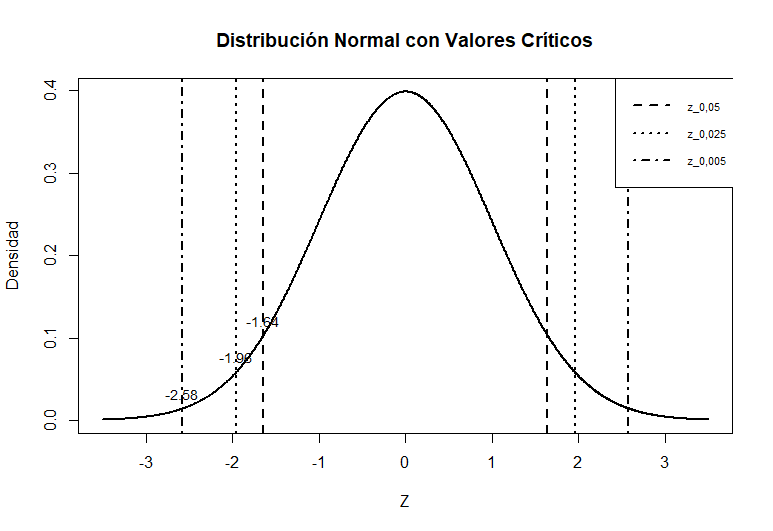
\includegraphics[width=0.9\linewidth]{normal_critic.png}
\end{figure}
 

\end{document}